\section{Introduction}
The main goal of this laboratory assignment is to design, implement and analyse a band-pass filter (BPF) using an OP-AMP (operational amplifier) having in mind that it should have a good relation efficiency-price. The final objective was to get a central frequency of $1kHz$ for the output signal and a voltage gain of $40dB$ and the circuit's efficiency will be measured considering these objectives that were set. \\

So, in order to evaluate the relation efficiency-price of the built circuit, we will use a merit figure that considers the total cost of the circuit and the deviation to the desired gain and central frequency, defined as:

\begin{equation}
    M = \frac{1}{cost \cdot |40 - gain| \cdot |1000 - central freq.|}
    \label{merit}
\end{equation}

To calculate the total cost associated to this circuit, one considered that it equals the sum of the cost of the resistors, capacitors and transistors which is given by:

\begin{table}[H]
    \centering
    \begin{tabular}{|c|c|}
        \hline
        \textbf{Component} &  \textbf{Price}\\
        \hline
        Resistors & 1 MU $k\Omega^{-1}$ \\ \hline
        Capacitors & 1 MU $\mu F^{-1}$ \\ \hline
        Transistors & 0.1 MU transistor$^{-1}$\\
        \hline
    \end{tabular}
    \caption{Price table for the components used}
    \label{tab:price}
\end{table}

The central frequency represented on eq. \eqref{merit} can be directly calculated from the definition of transfer function for this system and it is given by the geometric mean of the lower and higher cutoff frequencies:

\begin{equation}
    central freq. = \sqrt{f_H f_L}
\end{equation}

in which $f_H$ corresponds to the higher cutoff frequency and $f_L$ to the lower cutoff frequency. Finally, the value for the voltage gain used on eq. \eqref{merit} is easily obtained as the correspondent voltage value for the central frequency obtained. \\

The circuit used to implement this band-pass filter using an OP-AMP can be divided in 3 main regions as it can be seen on Fig. \ref{initialscheme}

\begin{figure}[H]
    \centering
    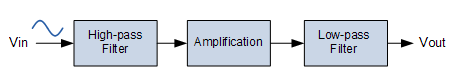
\includegraphics{esquemabunituh.PNG}
    \caption{Simplified scheme to present the 3 regions in which the circuit used can be divided}
    \label{initialscheme}
\end{figure}

The first part, a high-pass filter stage, will essentially have a resistor and a capacitor (i.e. will only pass signals with a frequency higher than a certain cutoff frequency, $f_L$). This part is followed by an amplification unit which will have the main objective of increasing the output voltage gain and which counts with an OP-AMP and two resistors. Finally, one implemented a low-pass filter stage on the circuit which operates on the opposite way of the high-pass filter, i.e. blocks all the signals with a frequency higher than a certain cutoff frequency, $f_H$). \\

As it is trivial, the high-pass filter and the low-pass filter blocking simultaneously frequencies lower than $f_L$ and higher that $f_H$ will act as a band-pass filter as desired. \\

Furthermore, and considering all the points mentioned before, the circuit used for this purpose was the following:


The results were obtained through a theoretical analysis, in which one predicted the output by using a theoretical method that suited the real circuit and through a simulation that was made using \textit{Ngspice}. The results obtained through both methods will be analysed throughout the report. However, because the models used in \textit{Ngspice} are more correct than the ones used on the theoretical analysis, any type of optimization was done almost exclusively in the simulation analysis.\\